\chapter{LHC-ATLAS実験}
\thispagestyle{empty}
\label{chap:2}
LHC-ATLAS~実験は、LHC(Large~Hadron~Collider)加速器を用いた陽子陽子衝突によって生成された粒子を~ATLAS~検出器を用いて測定する世界最大規模の素粒子実験である。標準模型の精密測定や新しい物理の探索を目的として行われている。
本章では、LHC~の概要及び~ATLAS~実験と各検出器について述べる。

\section{LHC 加速器}
スイスのジュネーブにある欧州原子核研究機構(CERN)の地下に建設された陽子陽子衝突型加速器(LHC)は、周長~27~km~のハドロンコライダーである。陽子バンチの衝突は~25~ns~おきに行われており、その頻度は~40~MHz~である。LHC~は陽子コライダーであるため、電子陽電子コライダーと比べ粒子がリング内を回る時のシンクロトロン放射光によるエネルギー損失が少ないことが特徴の一つである。トンネル内に多数の超伝導電磁石を並べて強力な磁場を作り出し、高エネルギーでの陽子陽子衝突を実現させる。

LHC~では、標準模型の精密検証や新物理の発見を目指した~ATLAS(A~Troidal~LHC~Apparatus)~\cite{URL:13}と~CMS(the~Compact~Muon~Solenoid)~\cite{URL:14}、重イオン衝突実験~ALICE(A~Large~Ion~Collider~Experiment)~\cite{URL:15}、フレーバー物理の~LHCb(Large~Hadron~Collider~beauty)~\cite{URL:16}の~4~つの実験が行われている。\figref{fig:lhc}は~LHC~全体の外観および各実験の衝突点について示したものである。

LHC~の運用スケジュールの詳細について説明する。LHC~は~2010~年から本格的な運転(Run~1)を開始した。Run~1~は~2010~年から~2012~年まで行われた。その後、2013~年から~2015~年初頭までの~LS1(Long~Shutdown~1)を経て~2018~年終わりまでの~Run~2~が施行された。そして二度目のアップグレード期間(LS2:Long~Shutdown~2)が~2021~年終わりまで取られ、2022~年から~Run~3~が行われる予定である。Run~3~の後には、より高いルミノシティでの~LHC~の運用が行われ、HL-LHC(High~Luminosity~LHC)として~2029~年から運転が施行される予定である。
ここでルミノシティとは、衝突型加速器における衝突点での粒子同士の衝突頻度を表している。\equref{eq:lumi}にルミノシティの定義を示す。
瞬間ルミノシティは一秒あたりの衝突頻度を表している。積算ルミノシティは瞬間ルミノシティを時間で積分したものとなる。観測されるデータ量は積算ルミノシティに比例し、積算ルミノシティの単位には~$\rm{fb}^{−1}$~が用いられる。
\tbref{tb:LHC}に各運転の詳細についてまとめる。
\begin{align}
    L = \frac{N}{\sigma} \label{eq:lumi}
\end{align}

\begin{table}[tb]
	\centering
	\begin{tabular}{c|cccc}\hline
	    \multirow{2}{*}{LHC Run} & \multirow{2}{*}{期~間} & 重心系エネルギー & 瞬間ルミノシティ & 積算ルミノシティ \\ 
	     &  & [TeV] & [$\rm{cm}^{-2}\rm{s}^{-1}$] & [$\rm{fb}^{-1}$] \\ \hline\hline
		Run 1 & 2010-2012 & 7-8 & $0.77\times10^{34}$ & $28.26$ \\ \hline
		Run 2 & 2015-2018 & 13 & $2\times10^{34}$ & $184.26$ \\ \hline
		Run 3 & 2022-2025 & 13.6 & $2\times10^{34}$ & 約$350$ \\\hline
		HL-LHC & 2029- & 14 & $5-7.5\times10^{34}$ & 約$3000-4000$
	\end{tabular}
	\caption[LHC の各運転における詳細]{LHC~の各運転における詳細~\cite{URL:18}~\cite{URL:17}。Run~3~以降については現在予定されている設定値を記している。積算ルミノシティは~LHC~で供給されるビームに基づいて計算している。}
    \label{tb:LHC}
\end{table}

\begin{figure}[H]
        \centering   
        \includegraphics[width=0.8\textwidth]{img/jpeg/lhclhc.pdf}
        \caption[LHC 加速器の全体像]{LHC~加速器の全体像~\cite{URL:01}。LHC~並びに~LHC~の前段加速器の詳細を示している。LHC~には、ATLAS,~ALICE,~CMS,~LHCb~の~4~つの検出器が設置されている。}\label{fig:lhc}
\end{figure}


\section{ATLAS~実験}
ATLAS~実験は~LHC~の衝突点に設置された~ATLAS~検出器を用いて陽子陽子衝突から~TeV~スケールまでの高エネルギー物理事象の探索を行う実験である。2012~年には、同じ~LHC~の~CMS~実験と共にヒッグス粒子を発見し、標準理論の完成に向けて大きく貢献した。
本節では、ATLAS~実験の詳細について記していく。
\subsection{ATLAS~検出器}
ATLAS~検出器は、直径~22~m、長さ~44~m~の円筒形で、総重量は~7000~t~という大型汎用検出器である。\figref{fig:atlasdet}に~ATLAS~検出器の全体図を示した。検出器は内側から内部飛跡検出器、電磁カロリメータ、ハドロンカロリメータ、ミューオン検出器という構成になっており、検出器の間には粒子を曲げるための超電導マグネットが設置されている。LHC~の高いルミノシティにおいても、様々な粒子の信号を無駄なく処理できるように、検出器は広範囲をカバーし、多様な検出器を組み合わせて利用することで高頻度の事象を逃すことなく処理するシステムが構築されている。\figref{fig:disp}は、衝突点より生成された粒子の各検出器における反応の様子を示したイベントディスプレイである。それぞれの検出器の特性をもとに各検出器で様々な粒子の識別を行う。

\begin{figure}[H]
    \centering   
    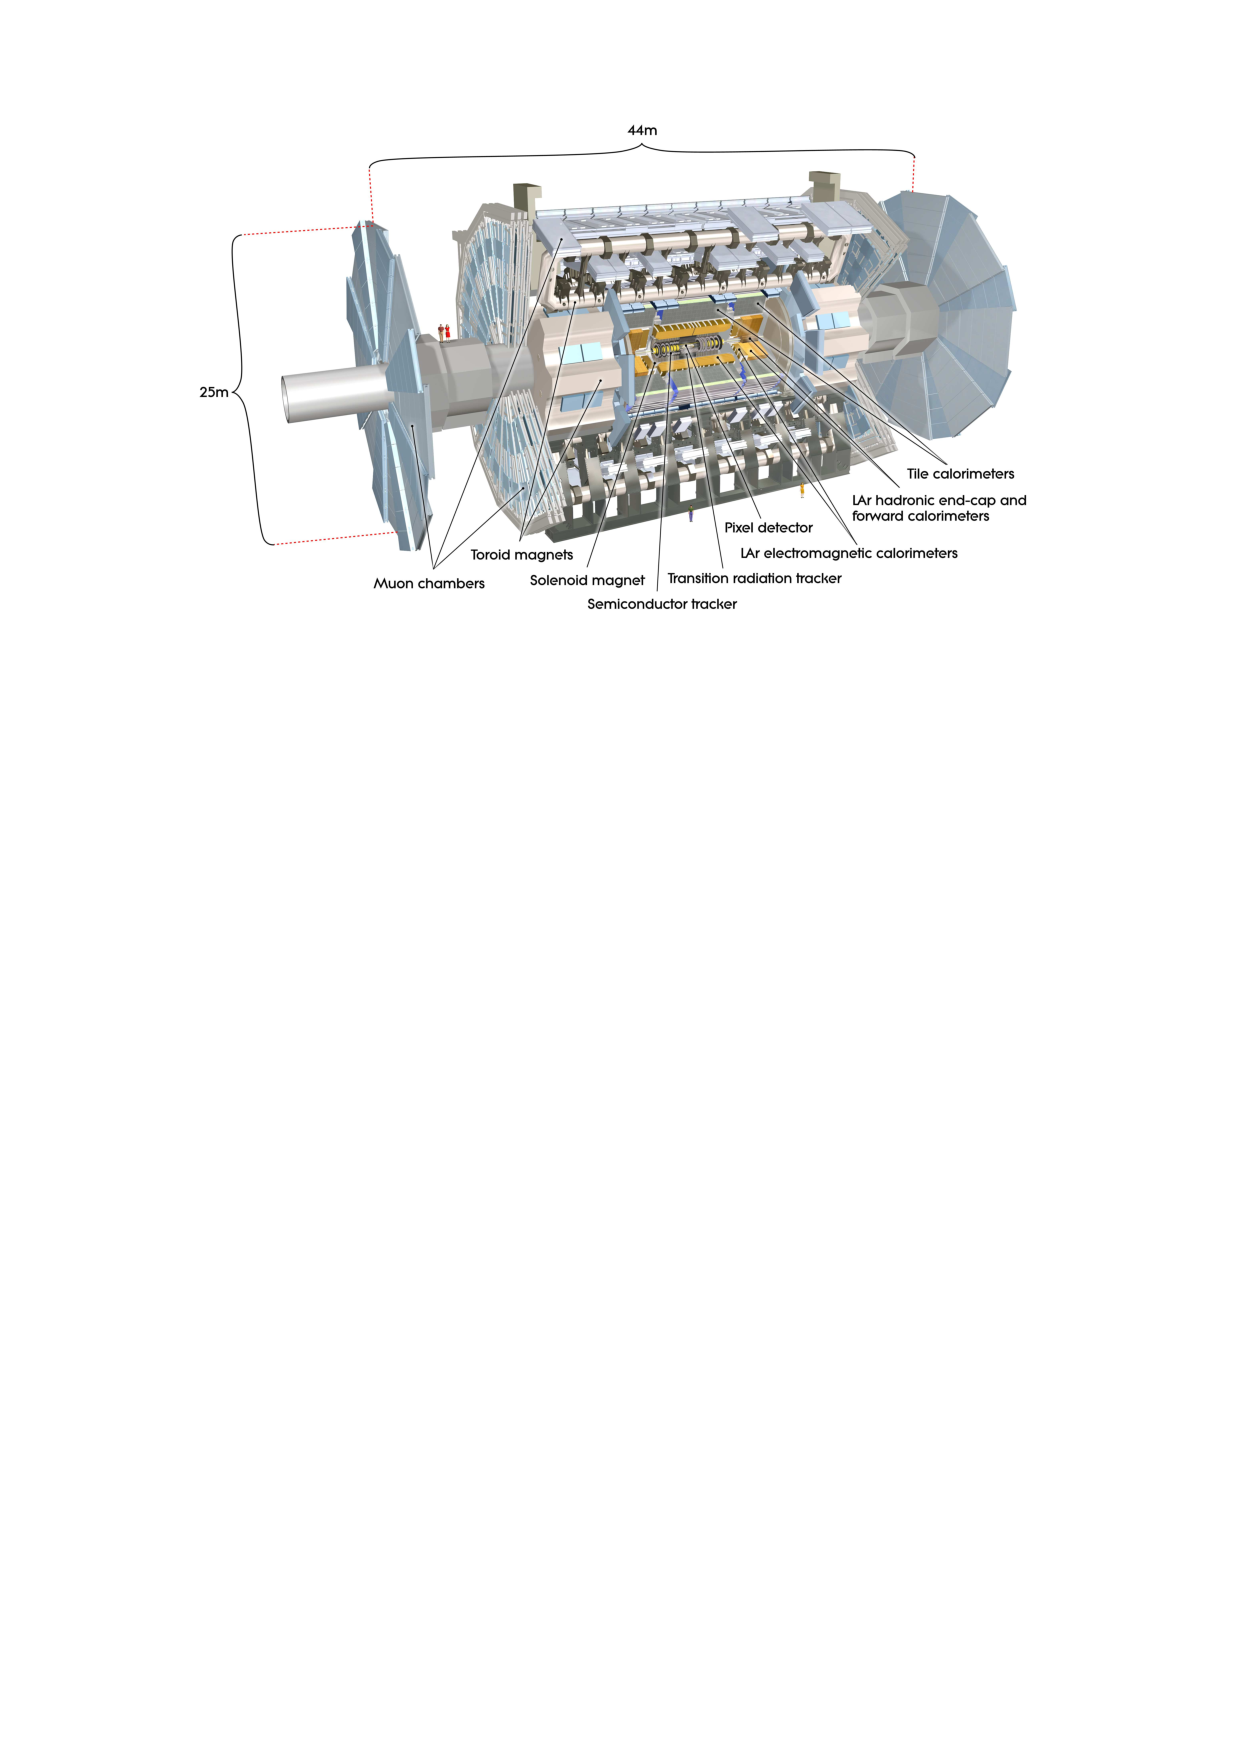
\includegraphics[width=0.9\textwidth,page=1]{img/pdf/ATLAS.pdf}
    \caption[ATLAS 検出器の全体図]{ATLAS 検出器の全体図~\cite{TR:01}。直径~25~m,~長さ~44~m,~重さ~7000~t~の大型汎用検出器。}\label{fig:atlasdet}
\end{figure}

\begin{figure}[htbp]
    \centering   
    \includegraphics[width=0.85\textwidth]{img/jpeg/how.png}
    \caption[ATLAS~検出器の断面図と通過する粒子のふるまい]{ATLAS~検出器の断面図と通過する粒子のふるまい~\cite{URL:02}。電磁カロリメータでは電子や光子、ハドロンカロリメータでは陽子や中性子、ミューオン検出器ではミューオンの検出を行う。}
    \label{fig:disp}
\end{figure}

\subsection{ATLAS~座標系}
ATLAS~で一般的に利用されている座標系について説明する。\figref{fig:cood}に~ATLAS~検出器のビーム衝突点を原点とした座標系を示した。直交座標系では検出器中心を原点にとり、ビーム軸方向を$~z~$軸、地面から垂直上方向を$~y~$軸、LHC~リングの中心を正方向を$~x~$軸として定義する。また、ATLAS~では検出器が円筒形のため極座標系が用いられることが多い。任意の$~z~$座標における動径方向を$~R$、方位角方向を~$\phi$、極角方向を~$\theta$~で表す。
また、$\theta$~方向を表す際には擬ラピディティ~$\eta$~というパラメータ、\equref{eq:eta}がよく用いられる。
擬ラピディティは、ローレンツ変換において不変であるため素粒子実験ではしばしば利用されるパラメータである。
擬ラピディティにより領域を区分することができ、ミューオン検出器においては、円筒型の側面部にあたる~$|\eta|<1.05$~をバレル領域、円筒型の底面部にあたる~$|\eta|>1.05$~をエンドキャップ領域($|\eta|>1.9$~をフォワード領域)
としている。また、$\eta~>~0$~の領域を~A-Side、$\eta~<~0$~の領域を~C-Side~と呼んでいる。

\begin{align}
    \eta = -\rm{ln}(\rm{tan}\frac{\theta}{2}) \label{eq:eta}
\end{align}

粒子のエネルギーや運動量を表す際には、ビーム軸に垂直な成分である横方向エネルギー~($E_{\rm{T}}$)、横方向運動量~($p_{\rm{T}}$)~を利用する。陽子陽子衝突実験において、衝突するクォークやグルーオンの$~z~$軸方向のエネルギー・運動量には陽子内のパートン分布により不定のため保存則を用いることはできない。一方で、ビーム軸に垂直な方向にはエネルギーおよび運動量の保存則が成立する。従って~$E_{\rm{T}}$~や~$p_{\rm{T}}$~は解析において利用されることが多い。またビーム軸に垂直な方向成分の保存則を用いると、ニュートリノ等の~ATLAS~検出器で観測できなかった粒子によるエネルギーの~2~次元のベクトル和を得ることができる。この見えないエネルギーの和を消失横方向エネルギー(Missing~$E_{\rm{T}}$~:~MET,~$E^{\rm miss}_{\rm{T}}$)と呼ぶ。

\begin{figure}[H]
    \centering  
    \includegraphics[width=\textwidth,page=1]{img/pdf/cood.pdf}
    \caption[ATLAS~実験において使用される座標系]{ATLAS~実験において使用される座標系。$x,~y,~z$~方向に設定される直交座標系と~$R,~\phi,~\theta$~で定義される極座標系がある。$\theta$~方向を表す量として、擬ラピディティ~$\eta$~が利用される。$\eta~>~0$~を~A-Side、$\eta~<~0$~を~C-Side~と呼ぶ。}\label{fig:cood}
\end{figure}

\subsection{超伝導マグネット}
ATLAS~は~3~種類の巨大な超電導磁石により構成されている。\figref{fig:mag}に~ATLAS~検出器における超伝導マグネットの構成を示した。一つは中央のソレノイド磁石であり内部検出器の運動量測定に用いられる。流れる電流は~7.73~kA~で、発生する磁場は約~2~T~である。その周りを囲むバレル領域のトロイド磁石は、八回対称のリングで構成されており、円周方向の磁場を生成する。エンドキャップ領域のトロイド磁石も同様に円周方向の磁場を生成する。これらのトロイド磁石はミューオンの運動量を測定するために利用されている。流れる電流は~20.5~kA~で、発生する磁場は約~4~T~である。

\begin{figure}[H]
        \centering   
        \includegraphics[width=0.75\textwidth,page=5]{img/pdf/ATLAS.pdf}
        \caption[ATLAS~検出器における超伝導磁石の構成]{ATLAS~検出器における超伝導磁石の構成~\cite{TR:01}。衝突点付近のソレノイド磁石と外側のトロイド磁石で構成されている。トロイド磁場はエンドキャップ領域、バレル領域それぞれにおいて八回対称になるように設定されている。}\label{fig:mag}
\end{figure}


\subsection{内部飛跡検出器}
内部飛跡検出器~\cite{URL:19}はビーム衝突点に最も近い位置に設置され、ソレノイド磁石の内部に位置している。内側から順に、ピクセル検出器(Pixel)、シリコントラッカー(SCT)、遷移輻射トラッカー(TRT)の~3~つで構成されている。
~Pixel~は、最内層にある半導体検出器であり、高い位置分解能を持つ。SCT~はマイクロストリップと呼ばれる細長い有感領域をシリコン上に施した半導体検出器である。そして~TRT~は、半径~4~mm~のチューブ型検出器であり、トラッキングのほかに遷移輻射を利用した電子の同定も行っている。
以上の内部飛跡検出器は、いずれもビーム衝突点に近く非常に厳しい放射線環境下にさらされるため、高い放射線耐性が必要不可欠である。\figref{fig:innr}は内部飛跡検出器の詳細を記した図である。

\begin{figure}[H]
    \centering   
    \includegraphics[width=0.95\textwidth,page=1]{img/jpeg/IDbriefing_figure1.png}
    \caption[ATLAS~検出器における内部飛跡検出器の構成]{ATLAS~検出器における内部飛跡検出器の構成~\cite{URL:19}。内側から順に~Pixel,~SCT,~TRT~検出器が設置されている。赤い星は、すべての検出器のヒットを示し、フィットされたトラックは黒い矢印で示される。青い線は、各レイヤーのトラックからヒットまでの差を表している。}\label{fig:innr}
\end{figure}

\subsection{カロリメータ}
カロリメータの主な役割は、電子やガンマ線、ジェット等のエネルギーおよび角度の測定である。ATLAS~実験に使用される~4~種類のカロリメータは、電磁カロリメータとハドロンカロリメータの~2~つのいずれかに区分され、広範囲をカバーしている。\figref{fig:calo}にカロリメータの構成を示した図を載せた。
以下では、それぞれのカロリメータについて簡単に説明する。

\begin{figure}[H]
        \centering   
        \includegraphics[width=0.8\textwidth,page=3]{img/pdf/ATLAS.pdf}
        \caption[ATLAS~検出器におけるカロリメータの構成]{ATLAS~検出器におけるカロリメータの構成~\cite{TR:01}。電磁カロリメータは、バレル領域およびエンドキャップ領域の~2~種類。ハドロンカロリメータは、バレル領域のタイル、エンドキャップ領域、フォワード領域の液体アルゴンカロリメータの~3~種類。}\label{fig:calo}
\end{figure}

\subsubsection{電磁カロリメータ}
電磁カロリメータは、アコーディオン構造のからなる鉛の吸収体と液体アルゴンで構成される。放射線耐性に優れており、電子と光子の同定に使用されている。ソレノイド磁石の外側に設置され、バレル領域、エンドキャップ領域それぞれをカバーしている。

\subsubsection{ハドロンカロリメータ}
バレル領域では、鉄の吸収体とタイル状のシンチレータから構成されたタイルカロリメータが用いられている。放射線強度がより高いエンドキャップ領域では、銅の吸収体と液体アルゴンから構成されたカロリメータが使用されている。またさらに放射線強度の高いフォワード領域には、銅とタングステンの吸収体と液体アルゴンからなるカロリメータが設置されている。
以上のハドロンカロリメータは、電磁カロリメータの外側に設置されており、ハドロンの同定、エネルギー測定およびジェットの再構成を行う。


\subsection{ミューオン検出器}
終状態に荷電レプトンを含む事象は、ジェットを引き起こすハドロンなどに比べ、飛跡を再構成しやすく、測定装置で捕えやすい。特にミューオンは物質に対する透過力が高く、寿命が長いために~ATLAS~検出器の外側でもほかの検出器の影響を受けることなく検出することが可能である。ミューオン検出器は、飛跡の精密測定用の~MDT(Monitored~Drift~Tube)、CSC(Cathorde~Strip~Chamber)と、トリガー用の~RPC(Resistive~Plate~Chamber)、TGC(Thin~Gap~Chamber)の~4~種類で構成され、ATLAS~検出器の最外層に設置されている検出器である。\figref{fig:mud}に各ミューオン検出器の構成を示した。

MDT~はバレル領域とエンドキャップ領域の両方に設置され、直径~30~mm~のドリフトチューブによって構成されている。CSC~はフォワード領域の内側に設置されたストリップチェンバーである。 また~RPC~はバレル領域、TGC~はエンドキャップ領域をカバーするように配置されており、PRC~は~平行平板ガス検出器、TGC~は薄いギャップの~MWPC(Multi~Wire~Proportional~Chamber)である。ミューオン検出器の特徴の詳細に関しては、\tbref{tb:muon}に記した。

バレル領域において、ミューオン検出器は~3~層の筒状のステーション上に配置されている。またエンドキャップ領域では、3~つの円盤状のステーション上に配置されている。バレル、エンドキャップそれぞれにビーム衝突点に近い方から、Inner,~Middle,~Outer~と呼んでいる。\figref{fig:tgc000}に~ATLAS~検出器における断面図と~TGC~検出器の配置を示した。TGC~は、Middle~に~M1,~M2,~M3~の~3~ステーション、トロイドマグネット内側の~Inner~に~EIFI~ステーションの合計~4~ステーションで構成されている。TGC~検出器における構成やエレクトロニクスに関する詳細は\chapref{chap:4}で述べる。

超電導トロイダル磁石はバレル領域およびエンドキャップ領域に検出器を内包するように配置され、それぞれ~$\phi$~方向の磁場を生成している。$\phi$~方向の磁場によって~R-Z~平面内で曲げられたミューオンの曲率を、バレル領域では~$\eta$、エンドキャップ領域では~$r$~によって測定し、その運動量を決定する。理想的にはミューオンは$~R-Z~$平面内で曲がるが、実際は磁場の大きさが一様でないため~$\phi$~方向にも曲がる。トリガー用の~2~つの検出器(RPC,~TGC)は、$\phi$~方向の座標を測る役割も担っている。

\begin{figure}[H]
        \centering   
        \includegraphics[width=0.7\textwidth,page=4]{img/pdf/ATLAS.pdf}
        \caption[ATLAS~検出器におけるミューオン検出器の構成]{ATLAS~検出器におけるミューオン検出器の構成~\cite{TR:01}。トリガー用の~RPC,~TGC~と精密測定用の~MDT,~CSC~で構成されている。}\label{fig:mud}
\end{figure}

\begin{figure}[H]
    \centering
    \includegraphics[width=0.8\textwidth,page=7]{img/slide/slide.pdf}
    \caption[Run~2~における~ATLAS~検出器を~$R-z$~方向から見たときの断面図および~TGC~各ステーションの配置]{Run~2~における~ATLAS~検出器を~$R-z$~方向から見たときの断面図および~TGC~各ステーションの配置~\cite{TR:01}。Big~Wheel~は、M1(3~層)、M2(2~層)、M3(2~層)の計~7~層で構成されており、Small~Wheel~は、EIFI(2~層)で構成されている。}\label{fig:tgc000}
\end{figure}

\begin{table}[tb]
	\centering
	\begin{tabular}{c|cccc}\hline
	    検出器 & 役割 & カバー領域 & 特徴 & チャンネル数 \\ \hline\hline
		\multirow{2}{*}{MDT} & トラッキング & \multirow{2}{*}{$0<|\eta|<3.0$} &\multirow{2}{*}{位置分解能 $\sigma_{\rm{x}}=60~ \mu \rm{m}$} & \multirow{2}{*}{約370000} \\ 
		& 運動量測定 & & & \\ \hline
		\multirow{2}{*}{CSC} & トラッキング & \multirow{2}{*}{$2.0<|\eta|<3.0$} &\multirow{2}{*}{位置分解能 $\sigma_{\rm{x}}=50~ \mu \rm{m}$} & \multirow{2}{*}{約67000} \\ 
		& 運動量測定 & & & \\ \hline
        \multirow{2}{*}{RPC} & \multirow{2}{*}{トリガー} & \multirow{2}{*}{$0<|\eta|<1.05$} &\multirow{2}{*}{時間分解能 $\sigma_{\rm{t}}=1~\rm{ns}$} & \multirow{2}{*}{約350000} \\ 
		&  & & & \\ \hline
        \multirow{2}{*}{TGC} & \multirow{2}{*}{トリガー} & \multirow{2}{*}{$1.05<|\eta|<2.04$} &\multirow{2}{*}{時間分解能 $\sigma_{\rm{t}}=4~\rm{ns}$} & \multirow{2}{*}{約320000} \\ 
		&  &  & \\ 
	\end{tabular}
	\caption{各ミューオン検出器における役割や特徴の一覧}
    \label{tb:muon}
\end{table}

\subsubsection{Run~3~におけるミューオン検出器のアップグレード}
初段ミューオンエンドキャップトリガーでは、\figref{fig:fake}で示したようなビームパイプから発生した陽子などの低速粒子による影響が課題となっていた。これらの粒子が高い~$p_{\rm{T}}$~を持つミューオンと同じ角度で入射した場合、誤ってトリガーを発行してしまう。2012~年に取得した~Run~1~の解析結果によると、初段エンドキャップミューオントリガーで出力されたうちの約~$90~\%$~がフェイクであった~\cite{TR:05}。その後の~Run~2~では、エンドキャップトロイドマグネットの内側に設置されたタイルカロリメータおよび~TGC~EIFI~とのコインシデンスを導入した。このようにインナーコインシデンスを要求することで、$1.05<|\eta|<1.92$~の領域におけるフェイクトリガーの削減に成功している。

しかし、$1.92<|\eta|<2.4$~の領域ではインナーコインシデンスを行うための検出器が設置されていないため、フェイクトリガーが多く残っており、$1.05<|\eta|<1.92$~の領域においてもフェイク削減の余地は残っている。そこで~Run~3~においてはさらなるフェイクトリガーの削減を目指し、トロイド磁場領域の内側に~NSW~(New~Small~Wheel)~および~RPC~BIS78~(RPC~Barrel~Inner~Small~sector~78)~の~2~つの検出器を新たに導入する。\figref{fig:innercoin}に示すように、Run~3~では~2~つの検出器の導入でさらなるフェイクトリガーの削減が可能であることが見積もられている。Run~3~における~新検出器導入後の~ATLAS~検出器の断面図を\figref{fig:cut3}に示した。

\figref{fig:nsw}に~NSW~の構成を示した。NSW~は$1.3<|\eta|<2.7$~の領域をカバーするガス検出器である。NSW~は、Run~2~で使用されていた~TGC~FI、MDT~EIL~チェンバー、CSC~と入れ替わる形で導入される。したがって、NSW~は~TGC~FI~が担っていたミューオントリガーの役割および~MDT~と~CSC~が担っていた飛跡の精密測定の役割を果たすこととなる。そのため、NSW~はトリガー検出器の役割を果たす~small~strip~TGC(sTGC)と主に飛跡の精密測定を行う~Micromegas(MM)で構成されている。NSW~を導入することでインナーコインシデンスの領域が~$|\eta|<2.4$~まで拡張される。

また\figref{fig:bis}には、RPC~BIS78~の構成を示した。Run~2~における問題点として、トロイドマグネットと干渉するため~TGC~EI~が設置できない領域が存在していたことが挙げられる。Run~3~では、この問題を解決するために、MDT~のBIS~チェンバーを~RPC~と~sMDT~(small~diameter~MDT)~を組み合わせた~RPC~BIS78~に置き換える。RPC~BIS78~は~$1.0<|\eta|<1.3$~の領域をカバーし、3~層のガス層で構成される。ガス層の厚みは約~1mm~で、従来の~RPC~の半分になっている。ガス層は従来の~RPC~と同様に~2~次元方向のストリップで~$\eta,~\phi$~方向が測定できる。

\begin{figure}[H]
        \centering   
        \includegraphics[width=0.7\textwidth,page=2]{img/pdf/trigger.pdf}
        \caption[L1~エンドキャップミューオントリガーにおけるフェイクトリガーの模式図]{L1~エンドキャップミューオントリガーにおけるフェイクトリガーの模式図~\cite{AR:02}。赤色の矢印はビームパイプから発生した低速粒子の軌道の例で、衝突点由来ではないフェイクミューオンの飛跡を表している。}
        \label{fig:fake}
\end{figure}

\begin{figure}[H]
        \centering   
        \includegraphics[width=0.7\textwidth,page=1]{img/pdf/inner.pdf}
        \caption[インナーコインシデンスによるフェイクトリガーの削減]{インナーコインシデンスによるフェイクトリガーの削減~\cite{TR:06}。Run~3~における初段ミューオントリガーを用いて選出したミューオン候補数の~$\eta$~分布の予測。タイル、RPC~BIS78~および~NSW~によって削減できるミューオン候補の数を示している。}
        \label{fig:innercoin}
\end{figure}

\begin{figure}[H]
        \centering   
        \includegraphics[width=0.8\textwidth,page=1]{img/pdf/bisbis.pdf}
        \caption[NSW~および~RPC~BIS78~が導入された~Run~3~における~ATLAS~検出器断面図]{NSW~および~RPC~BIS78~が導入された~Run~3~における~ATLAS~検出器断面図~\cite{TR:07}。}
        \label{fig:cut3}
\end{figure}

\begin{figure}[H]
        \centering   
        \includegraphics[width=0.8\textwidth,page=1]{img/pdf/nsw.pdf}
        \caption[New~Small~Wheel~の構成]{New~Small~Wheel~の構成~\cite{AR:14}。4~層の~sTGC~の間に、4~層$\times$2~の~MM~が挟まれる構造となっている。}
        \label{fig:nsw}
\end{figure}

\begin{figure}[H]
        \centering   
        \includegraphics[width=0.8\textwidth,page=1]{img/pdf/bis.pdf}
        \caption[RPC~BIS78~の構成]{BIS78~の構成~\cite{TR:04}。RPC~および~sMDT~で構成される。}
        \label{fig:bis}
\end{figure}

\section{ATLAS~トリガーシステム}\label{sec:ttri}
LHC~での陽子陽子衝突から生成される粒子は~ATLAS~のトリガーシステムを介して選別される。
陽子がクオークとグルーオンとの複合粒子であることと、高いルミノシティであることから、莫大な量のバックグラウンドが予想され、物理解析のために必要な情報をいかに効率よく正確に選別できるかがカギを握る。

ATLAS~実験の高頻度(40~MHz)陽子バンチ衝突に対して、最終的にデータとしての記録を許容できるイベントレートは数~kHz~である。この制限を満たし効率よくトリガーを行うために、ATLAS~実験ではハードウェアベースの初段トリガー~(Level-1~Trigger~:~L1)~とソフトウェアベースの後段トリガー~(High~Level~Trigger~:~HLT)~が実装されている。
\figref{fig:trigger}において、ATLAS 実験におけるトリガーと読み出し処理の流れについて示す。
本節では、ATLAS~実験におけるトリガーシステムについて詳しく説明する。

\begin{figure}[H]
        \centering   
            \includegraphics[width=\textwidth,page=2]{img/pdf/tdaq-run3-schematic-withoutFTK.pdf}
        \caption[Run~3~における~ATLAS~トリガーシステムの流れ]{Run~3~における~ATLAS~トリガーシステムの流れ~\cite{URL:07}。L1~では~$2.5~\mu\rm{s}$~以内にイベントレートを~$100~\rm{kHz}$~にまで削減する。L1~には、L1Calo,~L1Muon,~L1Topo~の~3~種類が存在する。HLT~ではソフトウェアベースでより詳細にトリガーを行い、数秒以内にイベントレートを数~kHz~にまで削減する。}\label{fig:trigger}
\end{figure}

\subsection{初段トリガー}\label{subsec:l1tri}
\subsubsection{初段トリガーでの処理の流れ}
初段トリガー(L1)におけるデータ処理の流れについて説明する。
\figref{fig:pipe}に~L1~における情報処理の流れを示した。L1~でのトリガー処理は、トリガー用ミューオン検出器(RPC,~TGC)およびカロリメータによって行われる。それぞれの検出器によって検出された~40~MHz~の頻度で繰り返される陽子バンチ衝突からのヒット信号は、25~ns~おきにL1~バッファに保持され、トリガー処理は情報が保持されている間に行われる。L1~の判定には最大~$2.5~\mu\rm{s}$~の時間がかかるため、L1~バッファでは最低~100~陽子バンチ分($25~\rm{ns}~\times~100~=~2.5~\mu\rm{s}$)のデータが保持できるように設定されている。そして決められた遅延時間~(Fixed~Latency)~を経たバンチ衝突のデータに対して、同一のバンチ衝突に対応した~L1~からの信号を受信し、情報の読み出しが行われる。以上のようなトリガー処理システムをパイプライントリガーと呼ぶ。L1~でのイベントの許容レートは~100~kHz~までに設定されており、以上のシステムを通じて~40~MHz~から~100~kHz~以下にまでレートを削減する。

カロリメータおよびミューオン検出器における~L1~の流れについて説明する。カロリメータトリガーでは、電子、光子、MET、タウ、ジェットの中から高い~$E_{\rm{T}}$~を持つ事象、ミューオントリガーでは、高い~$p_{\rm{T}}$~のミューオンヒットを持つ事象に対してトリガーを行う。L1~は、カロリメータの情報を用いて発行されるトリガー(L1Calo)、ミューオン検出器の情報を用いて発行されるトリガー(L1Muon)、それらを組み合わせた複合的なトリガー(L1Topo)の~3~種類に分類される。L1~では、まずカロリメータおよびミューオン検出器の情報から単独に事象選別を行う。また、ミューオントリガーはバレル領域とエンドキャップ領域で別々に処理が行われる。L1~Muon~の情報は~MUCTPI(Muon~to~CTP~Interface)へ送信され、事象の情報がまとめられる。
そして~L1Calo~と~MUCTPI~でまとめられた~L1Muon~の情報は、CTP(Central~Trigger~Processor)へと渡され、それぞれ処理が行われる。

また、L1Calo~と~L1~Muon~の情報は同時に~L1Topo~に送信され、複合的な情報処理が行われる。
L1Topo~においては~L1Calo~と~L1Muon~のトリガーアイテムを組み合わせたトリガーが発行できるだけでなく$\eta$~方向、$\phi$~方向の位置情報を用いて不変質量を組み、粒子の共鳴に由来することの要求も行うことができる。そして、L1Topo~で処理された情報についても、L1Muon~や~L1Calo~と同様に~CTP~へと送信される。

L1Calo,~L1Muon~および~L1Topo~の情報は、以上の流れから~CTP~に集められ、100~kHz~に収まるようにプリスケールがかけられたのちトリガー処理が行われる。CTP~で処理が行われ、データ読み出しが認められた信号に対しては~L1A(Level~1~Accept)が発行される。発行された~L1A~は~40~MHz~のクロックとともに~TTC(Timing~Trigger~and~Control)システムを経由して各測定器の読み出しシステムに送信される。

L1A~が発行された事象の信号は、情報の読み出しおよび保存を行うために~ROD(Read~Out~Driver)に送信される。このときデータは圧縮され、信号の情報とともに~BCID(バンチ交差識別番号:Bunch~Cross~Identification)と~EVID(イベント識別番号:Event~Identification)が付与される。BCID~は、LHC~の~25~ns~毎のバンチ衝突に対して、どのバンチに対応しているのかを識別する役割を持つ。EVID~は、生成粒子のイベントを識別するために付与される。ROD~は収集したデータをイベントごとに処理し、BCID~および~EVID~の整合性を確認し、S-LINK~\cite{URL:20}(Simple~Link~Interface)を通して、ROS(Read~Out~System)へと情報を送信する。

また、初段トリガーが発行された周辺の位置情報~(RoI~:~Region~of~Interest)~は、後段トリガーに渡され事象選別の種として利用される。

\subsubsection{初段トリガーにおけるタイミング合致の重要性}
前節で述べたように~L1~ではパイプライントリガーと呼ばれるシステムを採用している。このトリガーシステムにおいては、異なる検出器ごとの情報を同一のバンチ衝突ごとに対応させ、正しく一致させることが非常に重要となる。検出器は衝突点から最大で約~20~m~の距離に設置されておりミューオンの飛来時間は最大で約~100~ns~程の時間がかかるため、各検出器でタイミングをそろえるには、詳細な見積もりが必須である。L1Muon~および~L1Calo~では、各検出器に対し粒子がほぼ光速で到達するということを仮定した上で、基準に定めた陽子バンチ衝突による生成粒子の信号と判断した場合にトリガー判定を行っている。本論文では、トリガー判定を行う上で基準に定められたバンチのことを基準バンチ(Current~Bunch)と呼ぶこととする。L1Muon~や~L1Calo~では、基準バンチ由来ではないと考えられるタイミングでの入力情報に対しては、トリガー判定を行うことができない。一方、複合的なトリガーである~L1Topo~においては処理が特別であり、基準バンチの情報に加えて、その次のバンチの情報を組み合わせたトリガー判定を行うことが可能である。本論文では、基準バンチの次の陽子バンチ衝突のことを次のバンチ(Next~Bunch)、また基準バンチの前の陽子バンチ衝突のことを前のバンチ(Previous~Bunch)と呼ぶ。

以上で述べたように、正しくトリガー処理を行うには各検出器での同一事象のヒット情報を一致させる必要がある。そして、一致を保証する上においては、バンチ判定のタイミングをそろえることが非常に重要である。

\begin{figure}[H]
        \centering   
        \includegraphics[width=0.95\textwidth,page=1]{img/pdf/pipe.pdf}
        \caption[L1~におけるトリガーシステムの詳細]{L1~におけるトリガーシステムの詳細。40~MHz~での検出器からの情報は~L1~バッファに一時的に保持され、L1~トリガーでの信号の出力を受けたのち、順番に~ROD~へと送信される。}\label{fig:pipe}
\end{figure}

\subsection{後段トリガー}
後段トリガー~\cite{AR:15}(HLT)では、初段トリガーで出力された~RoI~を種として、ソフトウェアベースのアルゴリズムでオフライン解析に近い粒子の再構成を行う。HLT~では内部飛跡検出器および~MDT~や~CSC~などの精密測定用ミューオン検出器、L1Calo~におけるカロリメータなどの情報を用いて、飛跡再構成および~$E_{\rm{T}}$,~$p_{\rm{T}}$~の計算をする。L1~で~100~kHz~にまで落とされたイベントレートを~HLT~では数~kHz~にまで削減する。

HLT~は~L1~とは異なり、数~10~ms~-~1~s~程の長い計算時間によって、より詳細にトリガー判定を行う。また大量のコンピューティングファームを並行して利用することで精密で膨大な計算を早い時間で行うことができる。HLT~のアルゴリズムは~PU(Processing Unit)と呼ばれる約~40000~個のアプリケーションからなる専用コンピューティングファームで実行される。各~PU~は一つの事象を数~100~ms~以内に処理できるように設計されている。PU~の一連の処理においては複数の特徴抽出アルゴリズムが実行される。HLT~において、事象がアクセプトされるとオフライン再構成のためにデータをストレージへ送信し、最終的には~CERN~コンピューティングセンターの~Tier-0~施設に保存される。
